% fig_seed_scatter.tex -- results example: ALL 5 gated seeds for the
% CogVideoX/projectile in-range grid (Figure 1 panel (a) only shows 2).
% Draft only. Data below is the real per-clip gated (R^2>=0.8) g_hat from
% results/e0_pilot_cogvideox.json, reproduced exactly (see CLAUDE.md
% Section 5, "E0 (CogVideoX-5B-I2V)"). Magnitudes plotted (sign flipped),
% matching Figure 1's own convention.
%
% seed 0: (5,11.41) (7,11.39) (9.8,11.40) (12,11.46) (15,11.41)
% seed 1: (5,11.37) (7,11.41) (9.8,11.34) (12,11.79) (15,11.44)
% seed 2: (5,13.33)                                              [n=1, not a cluster]
% seed 3: (5,11.83)        (9.8,11.98) (12,10.71) (15,10.45)
% seed 4: (5,7.31) (7,7.00) (9.8,6.80) (12,7.06) (15,15,7.22)

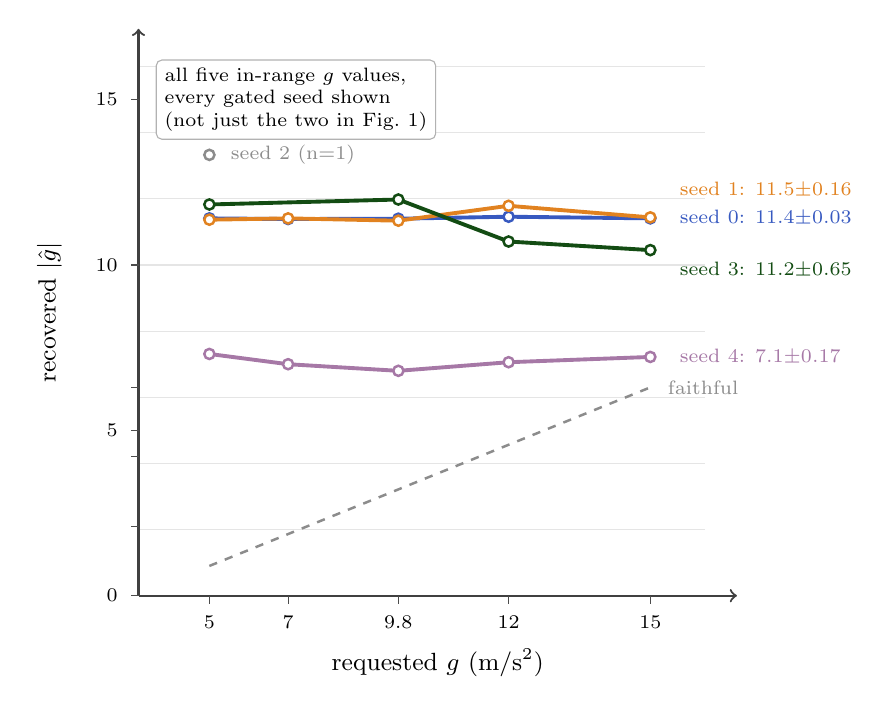
\begin{tikzpicture}[
  font=\small,
  ax/.style={->,thick,black!75},
  gridln/.style={black!10,line width=0.4pt},
  ideal/.style={dashed,black!45,line width=0.9pt},
  s0/.style={RoyalBlue!85!black},
  s1/.style={BurntOrange!90!black},
  s2/.style={black!45},
  s3/.style={ForestGreen!55!black},
  s4/.style={Plum!75!black},
  mk/.style={circle,inner sep=1.3pt,draw,line width=0.9pt,fill=white}
]

\foreach \y in {2,4,...,16}{\draw[gridln] (0,\y*0.42) -- (7.2,\y*0.42);}
\draw[ax] (0,0) -- (7.6,0);
\draw[ax] (0,0) -- (0,7.2);
\foreach \g/\x in {5/0.9,7/1.9,9.8/3.3,12/4.7,15/6.5}
  {\draw[black!70] (\x,0) -- (\x,-0.1); \node[font=\scriptsize,anchor=north] at (\x,-0.14) {\g};}
\foreach \v/\y in {0/0,5/2.1,10/4.2,15/6.3}
  {\draw[black!70] (0,\y*0.42*1) -- (-0.1,\y*0.42*1); \node[font=\scriptsize,anchor=east] at (-0.14,\y*0.42*1) {};}
\foreach \v in {0,5,10,15}
  {\draw[black!70] (0,\v*0.42) -- (-0.1,\v*0.42); \node[font=\scriptsize,anchor=east] at (-0.14,\v*0.42) {\v};}
\node[font=\small,anchor=north] at (3.8,-0.55) {requested $g$ (m/s$^2$)};
\node[font=\small,rotate=90,anchor=south] at (-0.85,3.6) {recovered $|\hat g|$};

% identity / faithful reference
\draw[ideal] (0.9,0.9*0.42) -- (6.5,6.3*0.42);
\node[black!45,font=\scriptsize,anchor=west] at (6.6,6.3*0.42) {faithful};

% seed 0
\draw[s0,line width=1.4pt] (0.9,11.41*0.42) -- (1.9,11.39*0.42) -- (3.3,11.40*0.42) -- (4.7,11.46*0.42) -- (6.5,11.41*0.42);
\foreach \x/\v in {0.9/11.41,1.9/11.39,3.3/11.40,4.7/11.46,6.5/11.41}{\node[mk,draw=RoyalBlue!85!black] at (\x,\v*0.42) {};}

% seed 1
\draw[s1,line width=1.4pt] (0.9,11.37*0.42) -- (1.9,11.41*0.42) -- (3.3,11.34*0.42) -- (4.7,11.79*0.42) -- (6.5,11.44*0.42);
\foreach \x/\v in {0.9/11.37,1.9/11.41,3.3/11.34,4.7/11.79,6.5/11.44}{\node[mk,draw=BurntOrange!90!black] at (\x,\v*0.42) {};}

% seed 3 (only 4 gated points)
\draw[s3,line width=1.4pt] (0.9,11.83*0.42) -- (3.3,11.98*0.42) -- (4.7,10.71*0.42) -- (6.5,10.45*0.42);
\foreach \x/\v in {0.9/11.83,3.3/11.98,4.7/10.71,6.5/10.45}{\node[mk,draw=ForestGreen!55!black] at (\x,\v*0.42) {};}

% seed 4
\draw[s4,line width=1.4pt] (0.9,7.31*0.42) -- (1.9,7.00*0.42) -- (3.3,6.80*0.42) -- (4.7,7.06*0.42) -- (6.5,7.22*0.42);
\foreach \x/\v in {0.9/7.31,1.9/7.00,3.3/6.80,4.7/7.06,6.5/7.22}{\node[mk,draw=Plum!75!black] at (\x,\v*0.42) {};}

% seed 2 (only 1 gated point, shown as a lone marker, not a cluster)
\node[mk,draw=black!45] at (0.9,13.33*0.42) {};
\node[font=\scriptsize,black!45,anchor=west] at (1.05,13.33*0.42) {seed 2 (n=1)};

% right-hand legend
\node[s0,font=\scriptsize,anchor=west] at (6.75,11.41*0.42) {seed 0: $11.4{\pm}0.03$};
\node[s1,font=\scriptsize,anchor=west] at (6.75,11.44*0.42+0.35) {seed 1: $11.5{\pm}0.16$};
\node[s3,font=\scriptsize,anchor=west] at (6.75,10.45*0.42-0.25) {seed 3: $11.2{\pm}0.65$};
\node[s4,font=\scriptsize,anchor=west] at (6.75,7.22*0.42) {seed 4: $7.1{\pm}0.17$};

\node[draw=black!30,fill=white,rounded corners=2pt,inner sep=3pt,font=\scriptsize,align=left]
  at (2.0,6.3) {all five in-range $g$ values,\\every gated seed shown\\(not just the two in Fig.~1)};

\end{tikzpicture}
